\chapter{Алгоритми зовнішнього сортування}


\nopagebreak[4]
\section{Вступ}
\nopagebreak[4]
\textbf{Зовнішнє сортування} - сортування даних, розташованих на периферійних пристроях і не вміщаються в оперативну пам'ять, тобто коли застосувати одну з внутрішніх сортувань неможливо. Варто відзначити, що внутрішня сортування значно ефективніше зовнішньої, так як на звернення до оперативної пам'яті витрачається набагато менше часу, ніж до магнітних дисків, стрічок і т.п.

Найбільш часто зовнішнє сортування використовується в СУБД.

Дані, що зберігаються на зовнішніх пристроях, мають великий обсяг, що не дозволяє їх цілком перемістити в оперативну пам'ять, відсортувати з використанням одного з алгоритмів внутрішнього сортування, а потім повернути їх на зовнішній пристрій. У цьому випадку здійснювалося б мінімальну кількість проходів через файл, тобто було б однократне читання і однократна запис даних. Однак на практиці доводиться здійснювати читання, обробку і запис даних у файл по блоках, розмір яких залежить від операційної системи та наявного обсягу оперативної пам'яті, що призводить до збільшення числа проходів через файл і помітного зниження швидкості сортування.

\section{Ключові терміни}
\nopagebreak[4]
\textbf{Зовнішнє сортування} - це сортування даних, які розташовані на зовнішніх пристроях і не вміщаються в оперативну пам'ять.

\textbf{Фаза} - це дії по одноразовій обробці всієї послідовності елементів.

\textbf{Серія (упорядкований відрізок)} - це послідовність елементів, що упорядкована по ключу. Кількість елементів в серії називається довжиною серії.

\textbf{Двофазне сортування} - це сортування, в якому окремо реалізується дві фази: розподіл і злиття. 

\textbf{Однофазне сортування} - це сортування, в якому об'єднані фази розподілу і злиття в одну.

\textbf{Двоколійним злиттям} називається сортування, в якому дані розподіляються на два допоміжних файли. 

\textbf{Багатоколійним злиттям} називається сортування, в якому дані розподіляються на N (N> 2) допоміжних файлів.



\section{Розширені теоретичні відомості}
\nopagebreak[4]

\subsection{Сортування простим злиттям}

Одне з сортувань на основі злиття називається простим злиттям.

Алгоритм сортування простим злиття є найпростішим алгоритмом зовнішньої сортування, заснований на процедурі злиття серією.

У даному алгоритмі довжина серій фіксується на кожному кроці. У вихідному файлі всі серії мають довжину 1, після першого кроку вона дорівнює 2, після другого - 4, після третього - 8, після k-го кроку - 2k.

Алгоритм сортування простим злиттям

\begin{enumerate}
\item Вихідний файл f розбивається на два допоміжних файлу f1 і f2.

\item Допоміжні файли f1 і f2 зливаються в файл f, при цьому поодинокі елементи утворюють впорядковані пари.

\item Отриманий файл f знову обробляється, як зазначено в кроках 1 і 2. При цьому впорядковані пари переходять у впорядковані четвірки.

\item Повторюючи кроки, зливаємо четвірки в вісімки і т.д., кожен раз подвоюючи довжину злитих послідовностей до тих пір, поки не буде впорядкований цілком весь файл (рис.~\ref{f:sort1}).
\end{enumerate}

\begin{figure}
\caption{Демонстрація сортування двоколійному двофазним простим злиттям}\label{f:sort1}
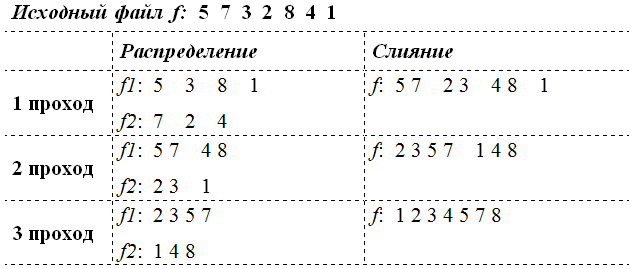
\includegraphics[width=13cm]{pic/43_01.png}

\end{figure}

Після виконання i проходів отримуємо два файли, що складаються з серій довжини 2i. Закінчення процесу відбувається при виконанні умови $2^i \geq n$. Отже, процес сортування простим злиттям вимагає порядку $O (\log n)$ проходів за даними.

Ознаками кінця сортування простим злиттям є наступні умови:

\begin{enumerate}
\item довжина серії не менша кількість елементів у файлі (визначається після фази злиття);
\item кількість серій рівно 1 (визначається на фазі злиття).
\item при однофазному сортуванні другий за рахунком допоміжний файл після розподілу серій залишився порожнім.
\end{enumerate}

Приклад програмної реалізації надано у додатку \ref{code:sort111};

\section{Приклади обчислень}
\nopagebreak[4]






